% BẢN NHÁP: văn bản do nhóm chỉnh sửa tại đây. Các chỗ @@TÊN@@ được src/make_report.py thay bằng số thật từ results/.
% Dán nội dung vào template của học phần nếu giảng viên yêu cầu (phần preamble có thể thay, thân bài giữ nguyên).
\documentclass[12pt,a4paper]{article}
% Biên dịch bằng XeLaTeX (Overleaf: Menu > Compiler > XeLaTeX). Latin Modern hỗ trợ đầy đủ tiếng Việt.
\usepackage{fontspec}
\setmainfont{Latin Modern Roman}
\usepackage[margin=2.5cm]{geometry}
\usepackage{booktabs,graphicx,float,amsmath,array,tikz,caption,hyperref}
\usetikzlibrary{positioning,arrows.meta}
\graphicspath{{figures/}}
\setlength{\parskip}{4pt}
\hypersetup{colorlinks=true,linkcolor=black,urlcolor=blue}
\renewcommand{\contentsname}{Mục lục}
\renewcommand{\figurename}{Hình}
\renewcommand{\tablename}{Bảng}
\renewcommand{\refname}{Tài liệu tham khảo}
\renewcommand{\appendixname}{Phụ lục}

\begin{document}

\begin{center}
{\large HỌC PHẦN NHẬP MÔN HỌC MÁY (FIT4013) -- NĂM HỌC 2026--2027}\\[6pt]
{\LARGE\bfseries BÁO CÁO BÀI TẬP LỚN}\\[8pt]
{\Large\bfseries Đề tài 8: Dự đoán sinh viên có nguy cơ bỏ học}\\[10pt]
Giảng viên: ThS. Lê Thị Thùy Trang\\[4pt]
Nhóm: [Họ tên -- MSSV thành viên 1], [Họ tên -- MSSV thành viên 2], [Họ tên -- MSSV thành viên 3]\\
Mã nguồn: [liên kết repository GitHub]
\end{center}

\tableofcontents
\newpage

% =====================================================================
\section{Đặt vấn đề và phân tích yêu cầu}
\subsection{Bối cảnh và mục tiêu}
Bỏ học đại học gây thiệt hại cho sinh viên, nhà trường và xã hội. Nếu nhận diện sớm được những sinh viên có nguy cơ bỏ học,
nhà trường có thể tư vấn học tập, hỗ trợ tài chính hoặc điều chỉnh lộ trình học kịp thời. Bài tập lớn xây dựng mô hình học máy
dự đoán kết quả học tập của sinh viên thuộc một trường đại học (nhãn \texttt{Target}) thành ba lớp: \textit{Dropout} (bỏ học),
\textit{Enrolled} (vẫn đang theo học) và \textit{Graduate} (tốt nghiệp).

Mục tiêu của nhóm gồm: (i) xây dựng quy trình học máy đầy đủ từ dữ liệu thô đến đánh giá; (ii) so sánh hai cách chuẩn bị dữ liệu
(Luồng A cơ bản, Luồng B cải tiến) trên ít nhất hai thuật toán đã học (K-NN, Cây quyết định, Naive Bayes); (iii) phân tích những
trường hợp mô hình dự đoán sai và rút ra khuyến nghị ứng dụng.

\subsection{Phân tích dữ liệu (EDA)}
\paragraph{Nguồn và cấu trúc.}
Dữ liệu là bộ ``Predict Students' Dropout and Academic Success'' \cite{realinho2022} gồm @@N@@ sinh viên, 36 đặc trưng và nhãn
\texttt{Target}. Không có giá trị thiếu và không có dòng trùng lặp. Các đặc trưng chia thành bốn nhóm: nhân khẩu học và gia đình
(tuổi, giới tính, hôn nhân, trình độ và nghề nghiệp của cha mẹ), thông tin tuyển sinh (ngành, hình thức xét tuyển, điểm đầu vào),
tài chính (nợ học phí, đóng học phí đúng hạn, học bổng) và kết quả học tập học kỳ 1, học kỳ 2 (số môn đăng ký, số lượt thi,
số môn đạt, điểm trung bình), cùng ba chỉ số kinh tế vĩ mô. Dựa vào số giá trị khác nhau, nhóm chia cột thành 8 cột nhị phân,
9 cột mã định danh (nominal, không có thứ tự như \texttt{Course}, \texttt{Application mode}, nghề nghiệp cha mẹ) và các cột số còn lại.

\paragraph{Phân phối nhãn.}
Nhãn mất cân bằng nhẹ: Graduate @@C_Graduate@@ sinh viên (@@P_Graduate@@), Dropout @@C_Dropout@@ (@@P_Dropout@@),
Enrolled @@C_Enrolled@@ (@@P_Enrolled@@) (Hình~\ref{fig:target}). Vì vậy nhóm dùng F1-macro làm thang đo chính, chia dữ liệu có
\texttt{stratify}, và không đánh giá mô hình chỉ bằng Accuracy.
\begin{figure}[H]\centering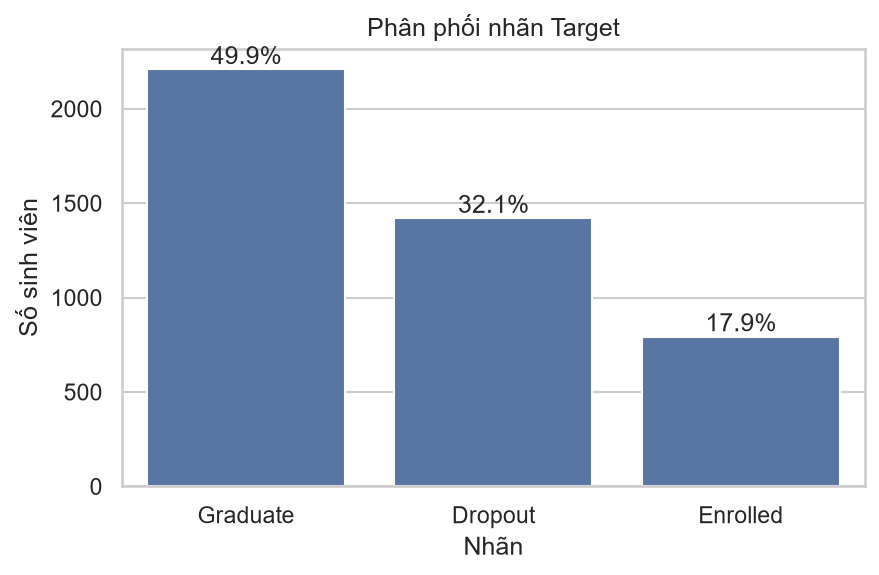
\includegraphics[width=0.5\textwidth]{eda_01_target.png}
\caption{Phân phối nhãn \texttt{Target}.}\label{fig:target}\end{figure}

\paragraph{Biến số và ngoại lệ.}
Các biến số chính (tuổi nhập học, điểm đầu vào, số môn đạt và điểm của hai học kỳ) được trực quan hóa bằng histogram và boxplot
theo nhãn (Hình~\ref{fig:hist}, \ref{fig:box}). Các biến học tập có nhiều giá trị bằng 0 và phân phối lệch; nhóm giữ nguyên các
ngoại lệ vì chúng phản ánh sinh viên thực (không thi, không đăng ký) chứ không phải lỗi nhập liệu.
\begin{figure}[H]\centering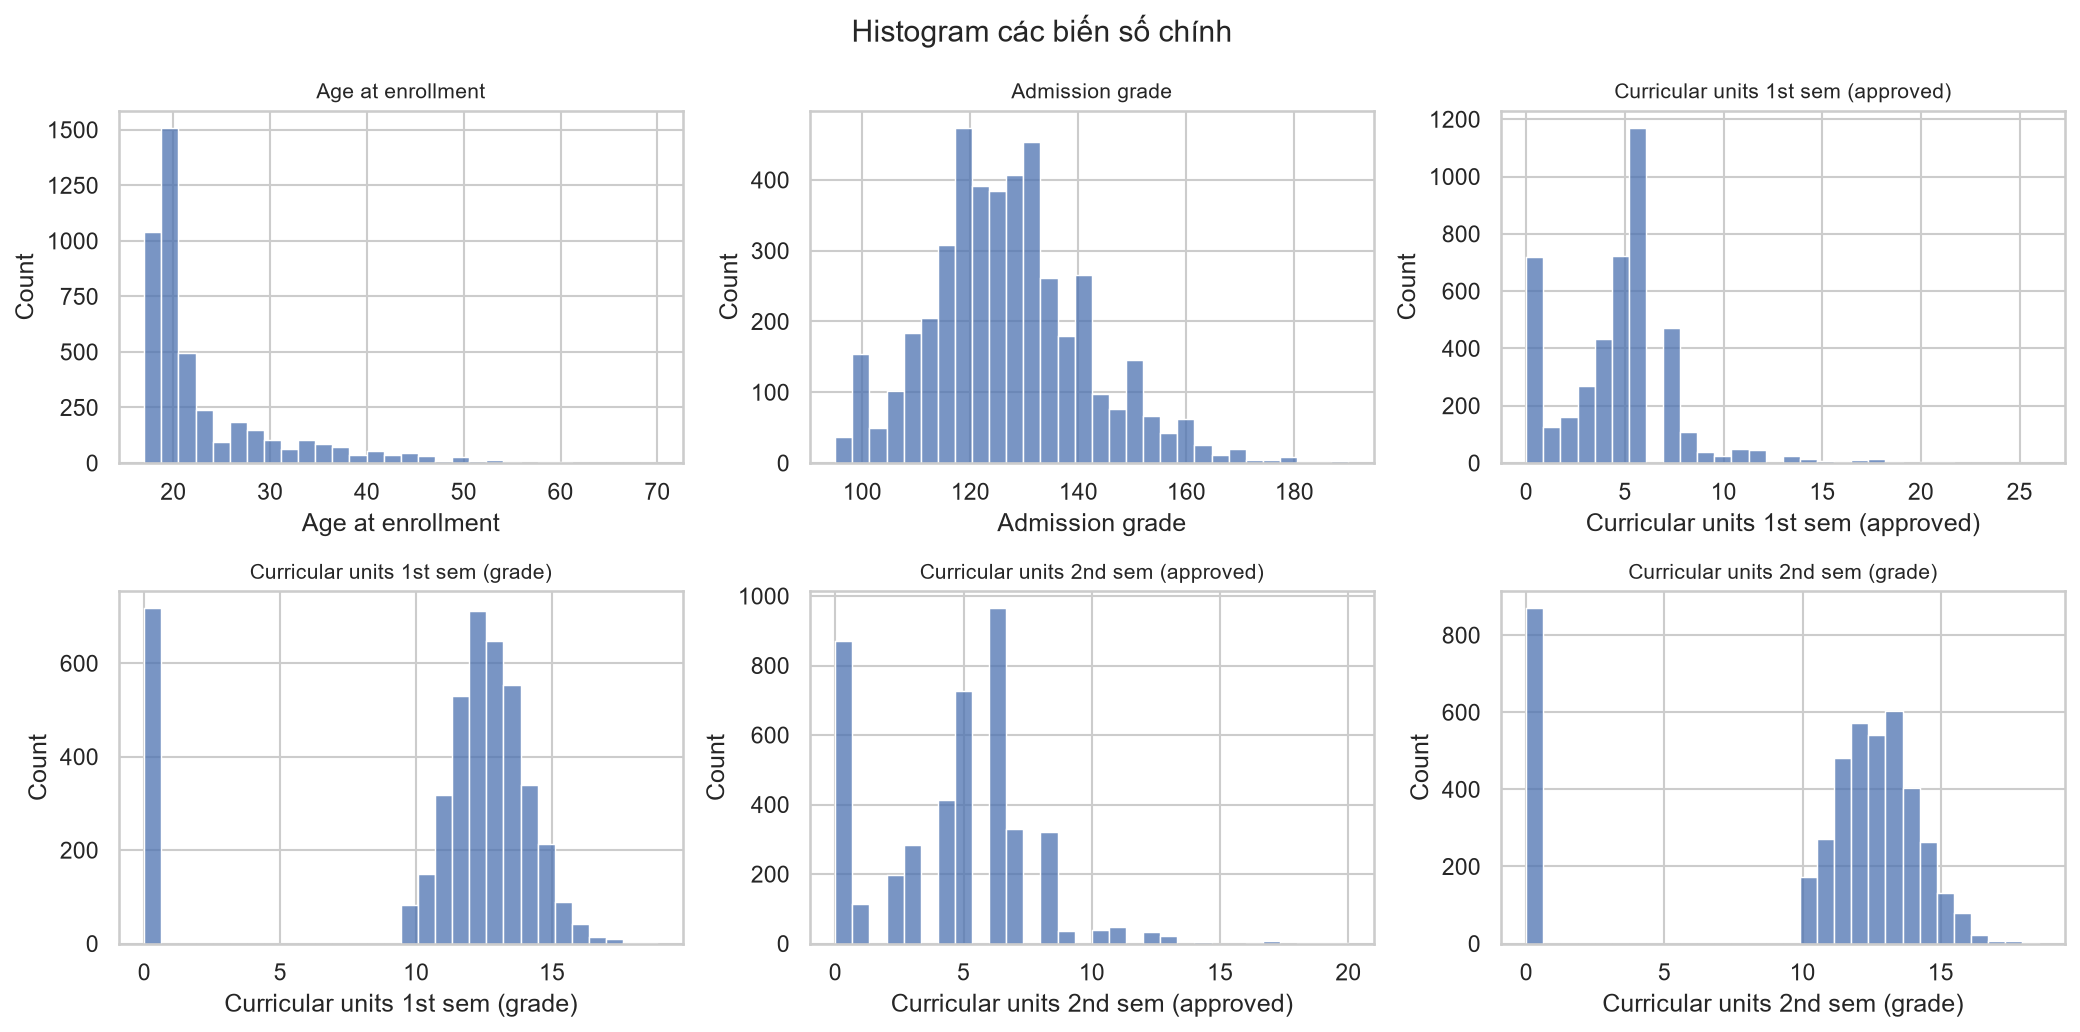
\includegraphics[width=0.95\textwidth]{eda_02_hist.png}\caption{Histogram các biến số chính.}\label{fig:hist}\end{figure}
\begin{figure}[H]\centering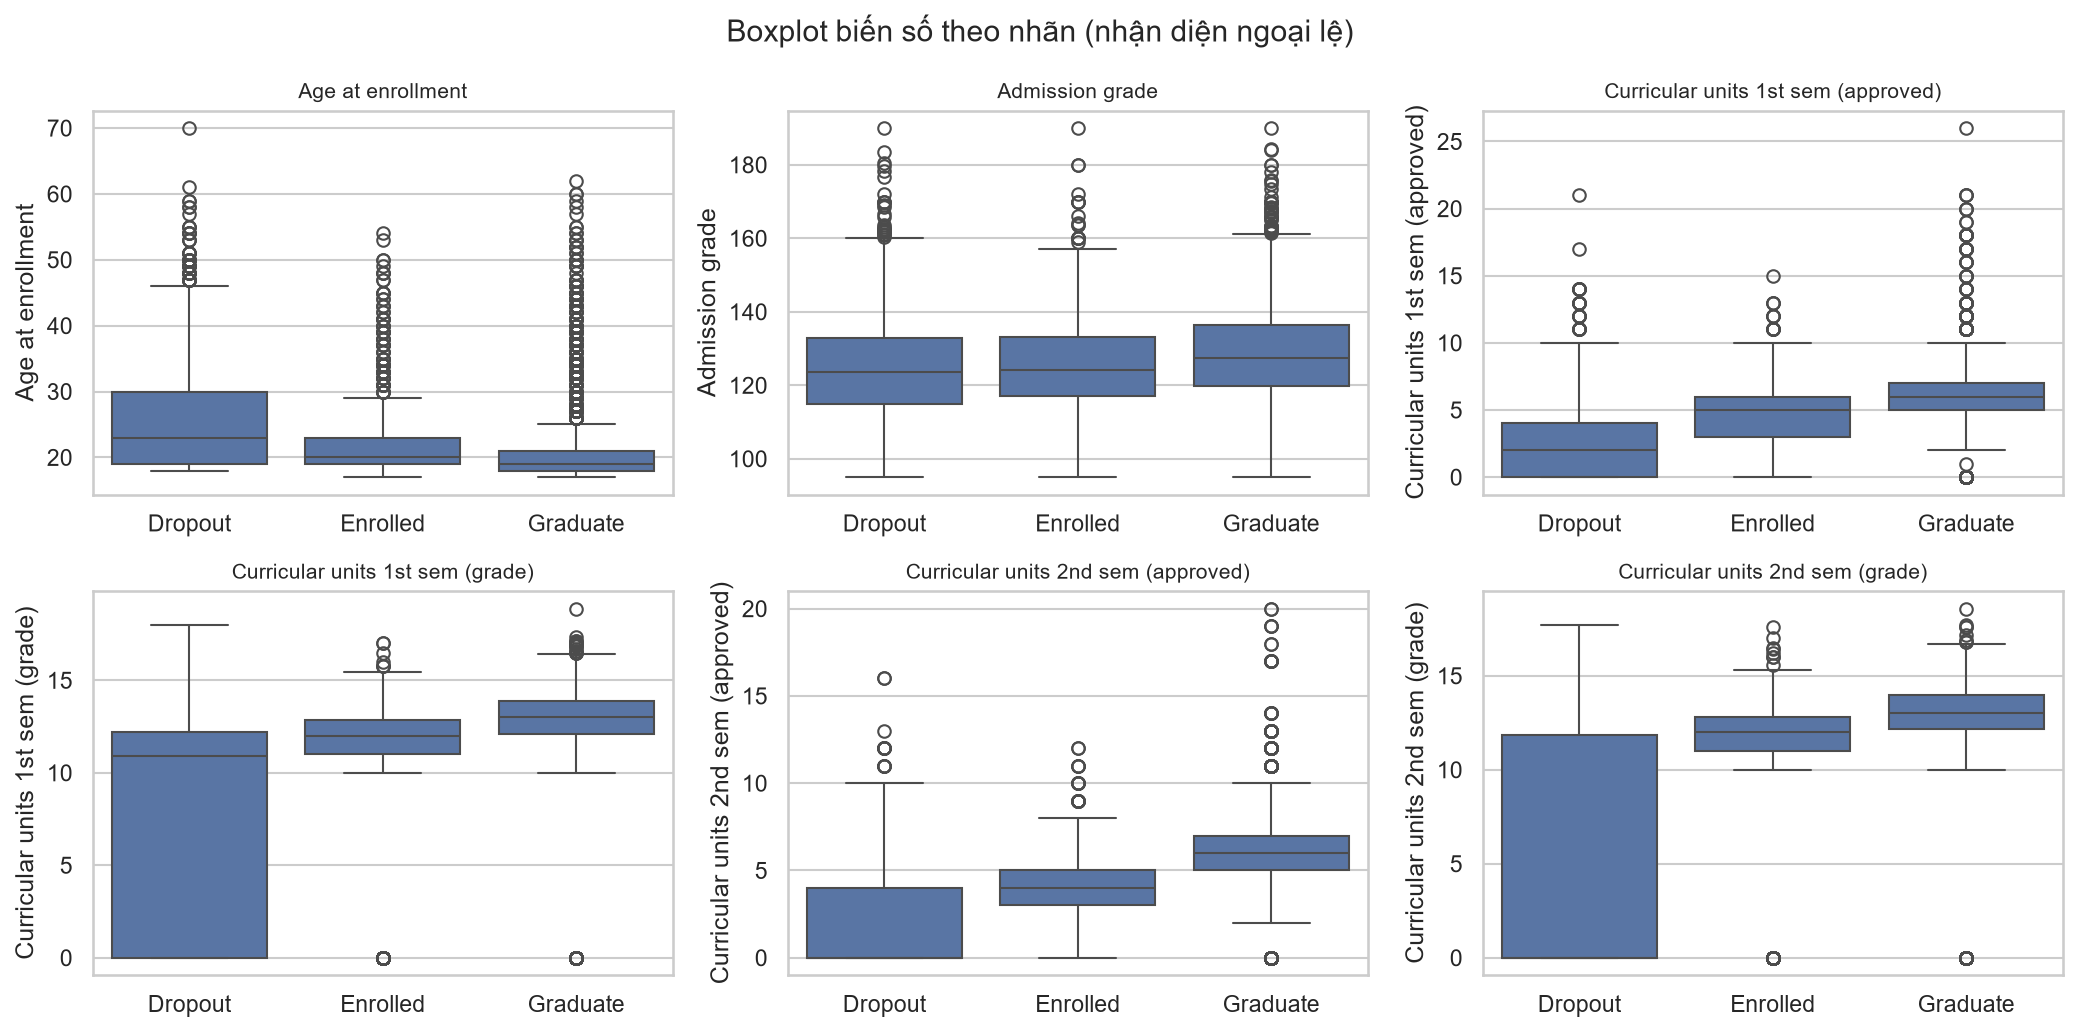
\includegraphics[width=0.95\textwidth]{eda_03_boxplot.png}\caption{Boxplot biến số theo nhãn.}\label{fig:box}\end{figure}

\paragraph{Tài chính và nhân khẩu học.}
Các biến tài chính phân tách nhãn rất rõ (Hình~\ref{fig:fin}). Tỷ lệ Dropout là @@FEE0@@ ở nhóm chưa đóng học phí đúng hạn so với
@@FEE1@@ ở nhóm đóng đúng hạn; @@DEB1@@ ở nhóm đang nợ so với @@DEB0@@ ở nhóm không nợ; @@SCH1@@ ở nhóm có học bổng so với @@SCH0@@
ở nhóm không có. Tỷ lệ Dropout của nhóm giới tính mã 1 là @@GEN1@@, của nhóm mã 0 là @@GEN0@@.
\begin{figure}[H]\centering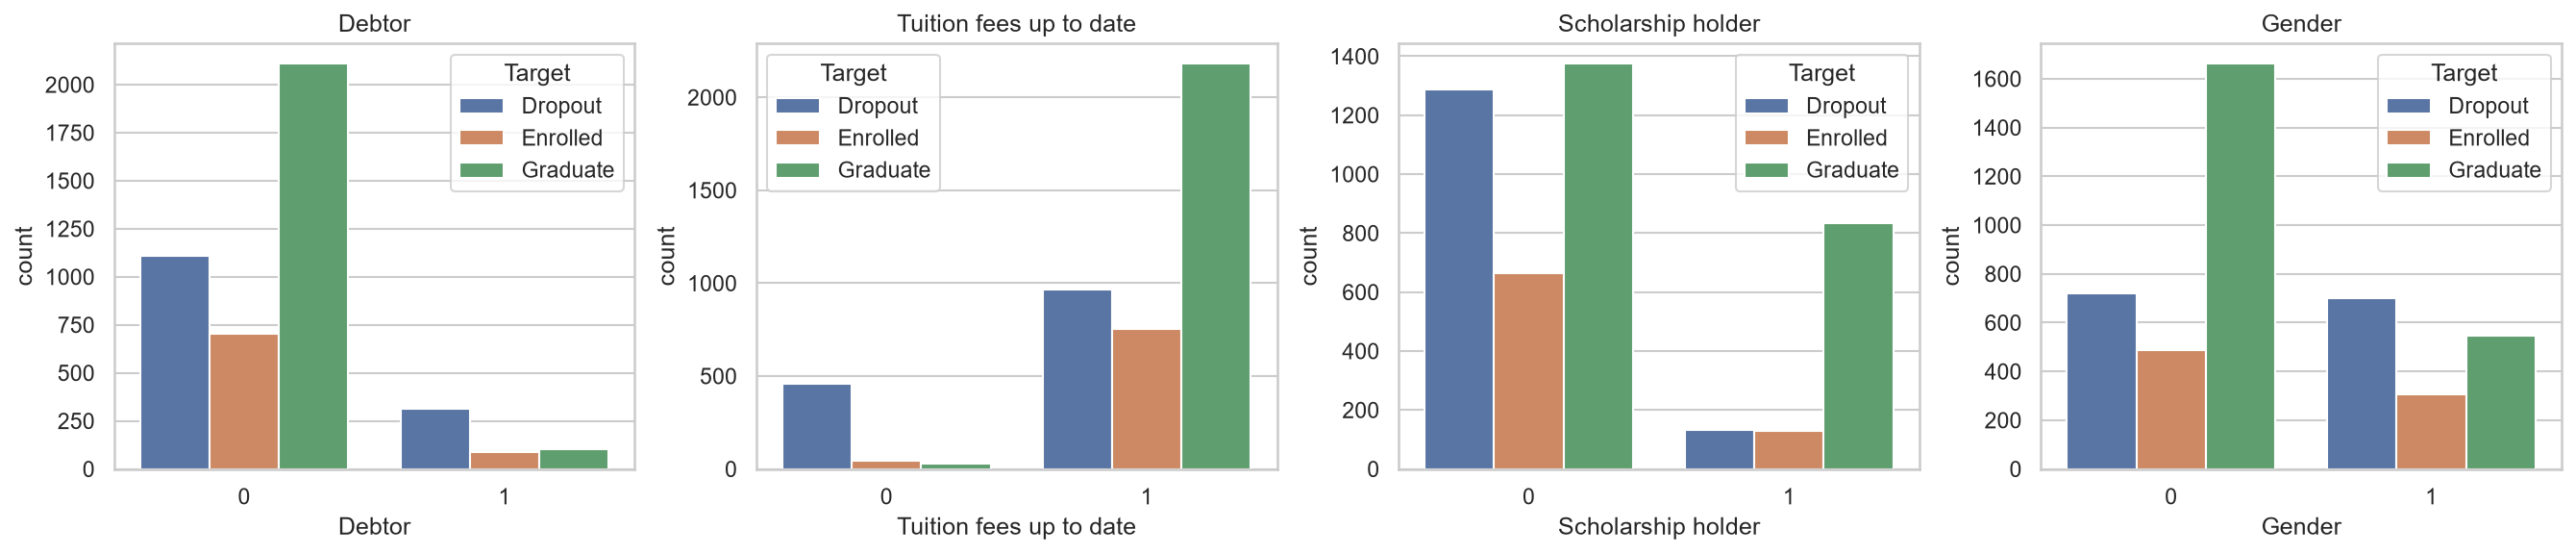
\includegraphics[width=\textwidth]{eda_04_financial.png}\caption{Biến tài chính và giới tính theo nhãn.}\label{fig:fin}\end{figure}

\paragraph{Tương quan.}
Trong các biến số, kết quả học tập có tương quan mạnh nhất với nhãn (mã hóa Dropout=0, Enrolled=1, Graduate=2):
số môn đạt học kỳ 2 (@@COR_A2@@), điểm học kỳ 2 (@@COR_G2@@), số môn đạt học kỳ 1 (@@COR_A1@@), điểm học kỳ 1 (@@COR_G1@@);
tuổi nhập học tương quan âm (@@COR_AGE@@). Các cặp biến học kỳ 1 và học kỳ 2 (đăng ký, đạt, điểm) tương quan rất mạnh với nhau
(Hình~\ref{fig:corr}), gợi ý tạo đặc trưng tỷ lệ ở Luồng B. Ngoài ra @@A2_ZERO_DROP@@ sinh viên Dropout không đạt môn nào ở học kỳ 2,
so với @@A2_ZERO_GRAD@@ ở nhóm Graduate.
\begin{figure}[H]\centering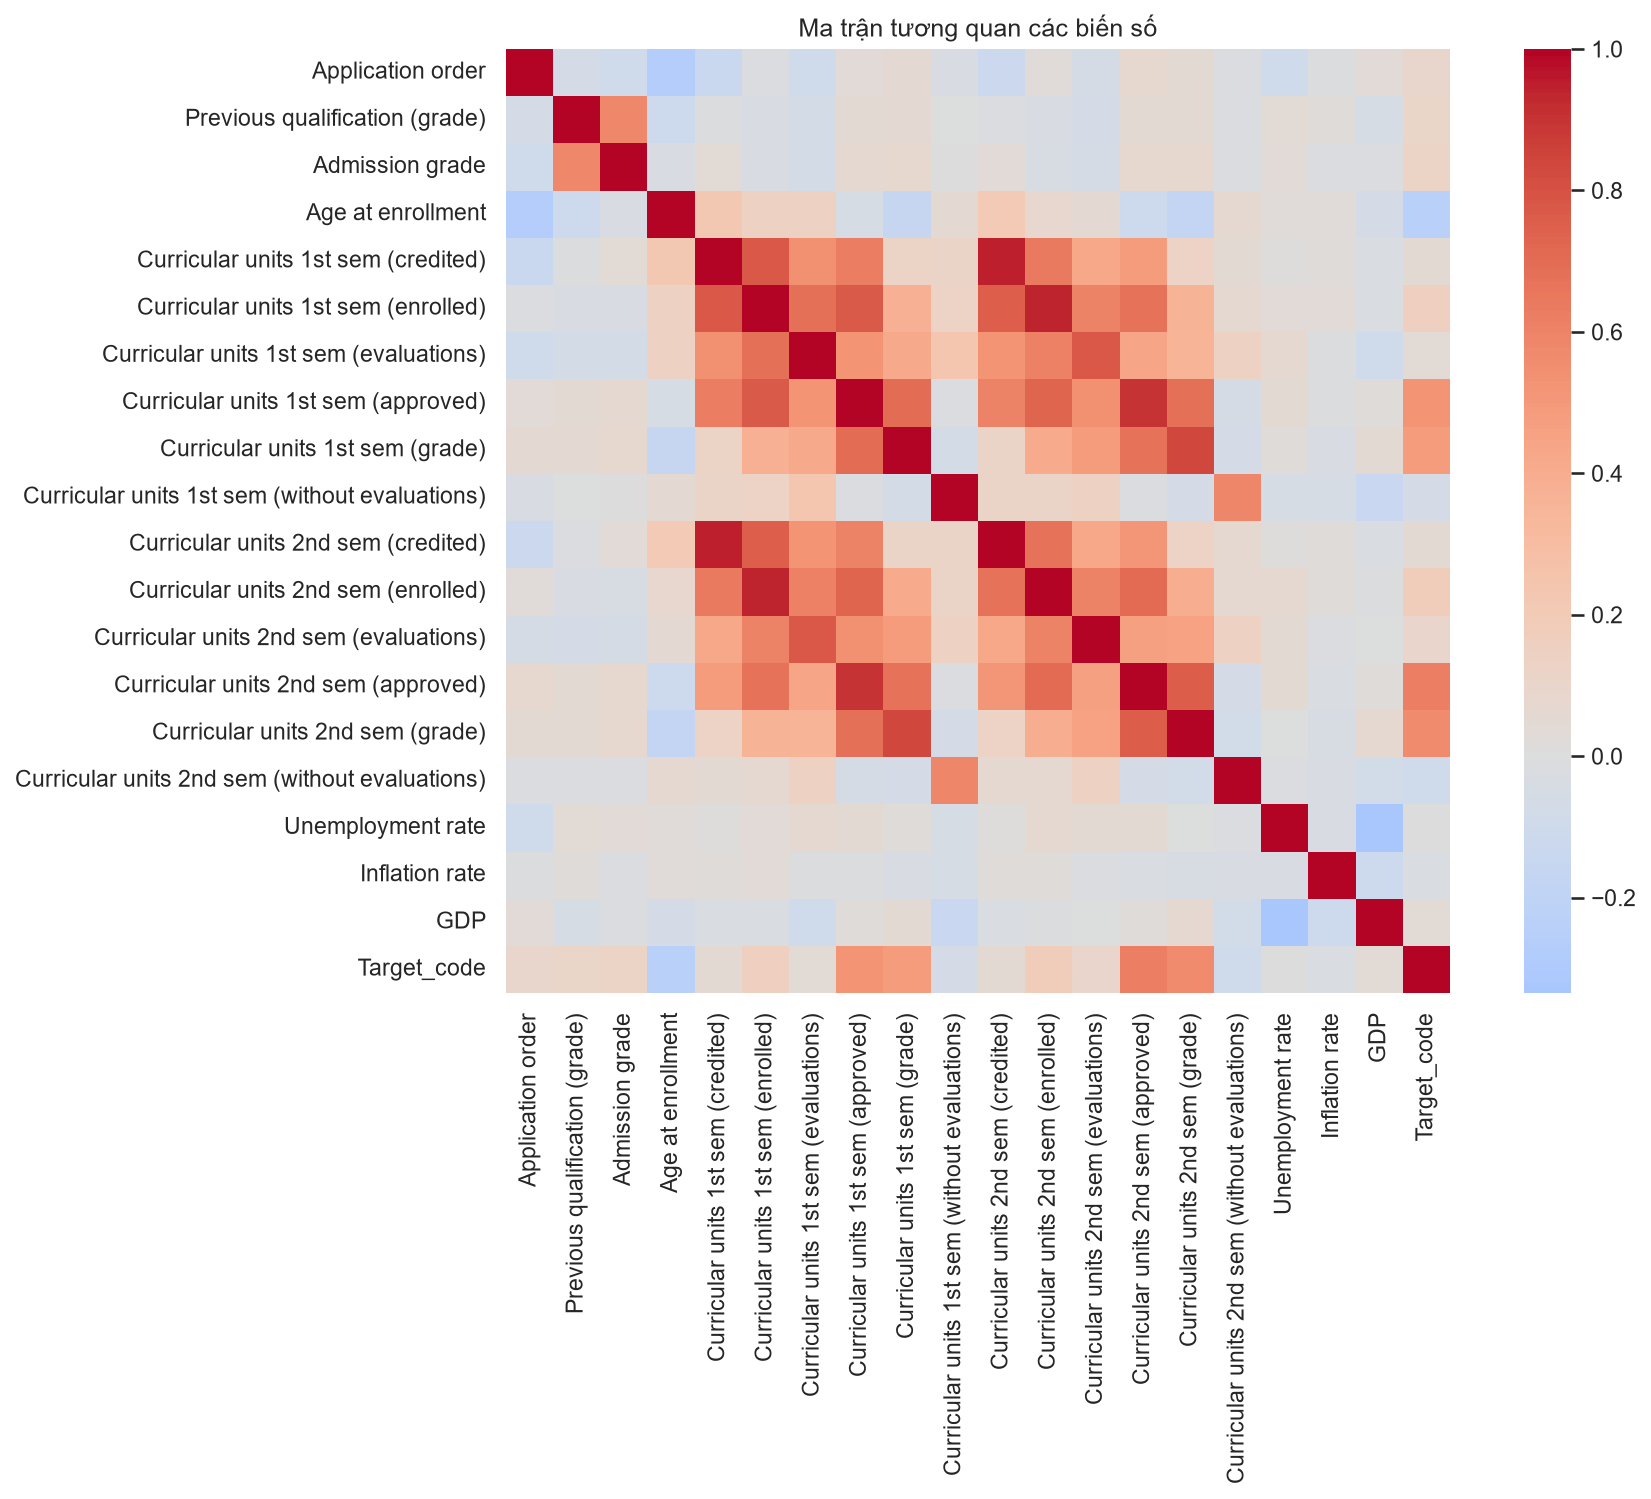
\includegraphics[width=0.8\textwidth]{eda_05_corr.png}\caption{Ma trận tương quan các biến số.}\label{fig:corr}\end{figure}

\paragraph{Dữ liệu bất thường.}
Có @@Z_G_N@@ sinh viên có điểm học kỳ 1 bằng 0; trong nhóm này @@Z_G_DROP@@ là Dropout, nên số 0 này là tín hiệu hữu ích và nhóm
giữ nguyên, không xóa hay điền bù. Có @@Z_E_N@@ sinh viên đăng ký 0 môn ở học kỳ 1, nhưng nhóm này phân bố gần như cân bằng
giữa Dropout (@@Z_E_DROP@@) và Graduate (@@Z_E_GRAD@@), tức là không thể coi ``0 môn đăng ký'' là dấu hiệu chắc chắn của bỏ học
(có thể là sinh viên được công nhận tín chỉ). Khi tính tỷ lệ ở Luồng B, các dòng có mẫu số bằng 0 cho kết quả 0.

% =====================================================================
\section{Thiết kế giải pháp và quy trình học máy}
\subsection{Sơ đồ quy trình}
\begin{figure}[H]\centering
\begin{tikzpicture}[box/.style={draw,rounded corners,align=center,minimum height=1.0cm,minimum width=2.1cm,font=\small},>=Stealth,node distance=0.45cm]
\node[box](a){Dữ liệu\\\texttt{data.csv}};
\node[box,right=of a](b){EDA};
\node[box,right=of b](c){Chia\\train/test};
\node[box,right=of c](d){Tiền xử lý\\(A hoặc B)};
\node[box,below=0.8cm of d](e){Huấn luyện\\+ GridSearchCV};
\node[box,left=of e](f){Đánh giá\\(test)};
\node[box,left=of f](g){Phân tích\\lỗi};
\node[box,left=of g](h){Kết luận};
\draw[->](a)--(b);\draw[->](b)--(c);\draw[->](c)--(d);\draw[->](d)--(e);\draw[->](e)--(f);\draw[->](f)--(g);\draw[->](g)--(h);
\end{tikzpicture}
\caption{Quy trình học máy của nhóm.}\end{figure}

\subsection{Chia dữ liệu và hạn chế data leakage}
Dữ liệu được chia train/test theo tỷ lệ 80/20 có \texttt{stratify} theo nhãn với \texttt{random\_state=42}, cho @@NTR@@ mẫu huấn luyện và
@@NTE@@ mẫu kiểm tra. Việc chọn mô hình và tham số chỉ dùng kết quả \texttt{StratifiedKFold} 5 lần (\texttt{shuffle=True},
\texttt{random\_state=42}) trên tập train với thang đo F1-macro; tập test chỉ dùng một lần để báo cáo. Mọi phép học tham số từ dữ liệu
(\texttt{StandardScaler}, \texttt{OneHotEncoder}) nằm trong \texttt{Pipeline} nên được fit lại trên phần train của mỗi lần CV, không
nhìn thấy dữ liệu kiểm tra. Các đặc trưng mới ở Luồng B được tính theo từng dòng, không dùng thống kê toàn tập, nên không gây rò rỉ.

\subsection{Hai luồng tiền xử lý}
Nhóm so sánh Luồng A và Luồng B từ cùng một dữ liệu thô. Để biết thay đổi nào thật sự có ích, nhóm thêm hai biến thể trung gian B1, B2
(ablation). Bảng~\ref{tab:flows} tóm tắt.
\begin{table}[H]\centering\small
\begin{tabular}{@{}lp{3.2cm}p{3.6cm}p{4.2cm}@{}}\toprule
Luồng & Mã định danh & Đặc trưng mới & Chuẩn hóa\\\midrule
A (cơ bản) & giữ nguyên dạng số & không & \texttt{StandardScaler} (K-NN, NB)\\
B1 & giữ nguyên dạng số & có & như A\\
B2 & One-Hot & không & như A\\
B & One-Hot (\texttt{min\_frequency}=20) & có & như A\\\bottomrule
\end{tabular}\caption{Các luồng tiền xử lý.}\label{tab:flows}\end{table}
Các đặc trưng mới (giả thuyết: tỷ lệ phản ánh mức độ hoàn thành tốt hơn số tuyệt đối, vì sinh viên đăng ký ít môn thì số môn đạt thấp một
cách tự nhiên): \texttt{approval\_rate} (môn đạt / môn đăng ký) và \texttt{eval\_pass\_rate} (môn đạt / lượt thi) cho từng học kỳ,
\texttt{grade\_delta} (điểm học kỳ 2 trừ học kỳ 1) và \texttt{total\_approved} (tổng môn đạt). Ví dụ \texttt{approval\_rate\_2nd}
có tương quan @@COR_RATE2@@ với nhãn, cao hơn cột gốc số môn đạt học kỳ 2 (@@COR_A2@@). Cột mã định danh được One-Hot vì các mã
(ngành, hình thức xét tuyển, nghề nghiệp) không có thứ tự, nên khoảng cách số học giữa các mã vô nghĩa với K-NN.

\subsection{Thuật toán và tham số}
Nhóm dùng ba thuật toán đã học, mỗi thuật toán có cấu hình mặc định (baseline) và cấu hình tinh chỉnh bằng \texttt{GridSearchCV}.
\begin{table}[H]\centering\small
\begin{tabular}{@{}lp{9.5cm}@{}}\toprule
Thuật toán & Lưới tham số\\\midrule
K-NN & \texttt{n\_neighbors} $\in\{3,5,7,11,15,21\}$; \texttt{weights} $\in\{$uniform, distance$\}$; \texttt{metric} $\in\{$euclidean, manhattan$\}$ (24 tổ hợp)\\
Cây quyết định & \texttt{max\_depth} $\in\{3,4,5,6,8,10,\text{None}\}$; \texttt{criterion} $\in\{$gini, entropy$\}$; \texttt{min\_samples\_leaf} $\in\{1,5,10,20\}$; \texttt{class\_weight} $\in\{\text{None},\text{balanced}\}$ (112 tổ hợp)\\
GaussianNB & \texttt{var\_smoothing} $\in\{10^{-9},10^{-7},10^{-5},10^{-3},10^{-2},10^{-1},1\}$\\\bottomrule
\end{tabular}\caption{Lưới tham số.}\end{table}
K-NN được chọn vì đơn giản, nhạy với cách biểu diễn đặc trưng (rất hợp để quan sát tác động của tiền xử lý); Cây quyết định dễ diễn giải
và xử lý tốt đặc trưng rời rạc; Naive Bayes là mốc xác suất nhanh. \texttt{class\_weight=balanced} được đưa vào lưới để xử lý mất cân bằng nhãn.

% =====================================================================
\section{Phân tích mã nguồn và chức năng}
Mã nguồn được tổ chức trong repository như sau (chạy từ thư mục gốc; xem \texttt{README.md}).
\begin{table}[H]\centering\small
\begin{tabular}{@{}lp{9.3cm}@{}}\toprule
Tệp & Chức năng\\\midrule
\texttt{src/data.py} & đọc \texttt{data.csv} (\texttt{sep=';'}, làm sạch tên cột), chia train/test, \texttt{StratifiedKFold}\\
\texttt{src/features.py} & đặc trưng mới của Luồng B (an toàn khi bỏ cột học kỳ 2)\\
\texttt{src/preprocess.py} & \texttt{make\_preprocessor(flow, scale)}: dựng Luồng A, B1, B2, B bằng \texttt{ColumnTransformer}\\
\texttt{src/models.py} & mô hình, lưới tham số, \texttt{make\_pipeline(flow, model)}\\
\texttt{src/evaluate.py} & Accuracy, Precision, Recall, F1 (macro và từng lớp), confusion matrix\\
\texttt{src/run\_experiments.py} & chạy toàn bộ thí nghiệm, ghi \texttt{results/}, \texttt{models/}, hình\\
\texttt{notebooks/01--04} & EDA, Luồng A, Luồng B (ablation), đánh giá và phân tích lỗi\\
\texttt{app.py}, \texttt{src/predict.py} & GUI demo (Streamlit) dùng mô hình đã lưu\\\bottomrule
\end{tabular}\caption{Cấu trúc chương trình.}\end{table}
Đoạn mã quan trọng nhất là hàm dựng tiền xử lý, nơi \texttt{OneHotEncoder} và \texttt{StandardScaler} được đặt trong \texttt{Pipeline}
(rút gọn):
\begin{small}\begin{verbatim}
def make_preprocessor(flow, scale):
    use_fe = flow in ("B", "B1")
    use_onehot = flow in ("B", "B2")
    scaler = StandardScaler() if scale else "passthrough"
    steps = []
    if use_fe:
        steps.append(("features", FunctionTransformer(add_features)))
    if use_onehot:
        onehot = OneHotEncoder(handle_unknown="ignore",
                               min_frequency=20, sparse_output=False)
        ct = ColumnTransformer([("onehot", onehot, _id_cols),
                                ("num", scaler, _non_id_cols)])
    else:
        ct = ColumnTransformer([("num", scaler, _all_cols)])
    steps.append(("columns", ct))
    return Pipeline(steps)
\end{verbatim}\end{small}
Và vòng tinh chỉnh tham số (chọn theo CV, test chỉ dùng để báo cáo):
\begin{small}\begin{verbatim}
gs = GridSearchCV(make_pipeline(flow, m), PARAM_GRIDS[m], cv=cv,
                  scoring="f1_macro", n_jobs=2, refit=True)
gs.fit(Xtr, ytr)                         # chỉ dùng tập train
best = gs.best_estimator_
metrics = evaluate(yte, best.predict(Xte))  # báo cáo trên test
\end{verbatim}\end{small}
Toàn bộ thí nghiệm chạy lại bằng một lệnh (\texttt{python src/run\_experiments.py}, khoảng 2 phút); cấu hình và phiên bản thư viện
được ghi trong \texttt{results/run\_info.json}.

% =====================================================================
\section{Thử nghiệm và kết quả}
\subsection{Thiết lập}
Chia 80/20 có \texttt{stratify} (\texttt{random\_state=42}); chọn tham số bằng CV 5 lần trên tập train theo F1-macro; báo cáo Accuracy,
F1-macro, Recall của Dropout (lớp cần phát hiện nhất) và F1 của Enrolled (lớp khó nhất). \textbf{Baseline} là cấu hình mặc định của từng
thuật toán trên Luồng A (K-NN $k=5$, Cây quyết định mặc định, GaussianNB mặc định); baseline được dùng làm mốc cho mọi so sánh.

\subsection{Kết quả chính}
\begin{table}[H]\centering\scriptsize
\resizebox{\textwidth}{!}{%
\begin{tabular}{@{}llllccccc@{}}\toprule
Thuật toán & Luồng & Mô hình & Tham số & CV F1-macro & Acc & F1-macro & Recall Dropout & F1 Enrolled\\\midrule
@@TABLE_MAIN@@
\bottomrule
\end{tabular}}\caption{Kết quả trên tập test (CV tính trên tập train; $\pm$ là độ lệch chuẩn giữa 5 fold).}\label{tab:main}\end{table}

\begin{figure}[H]\centering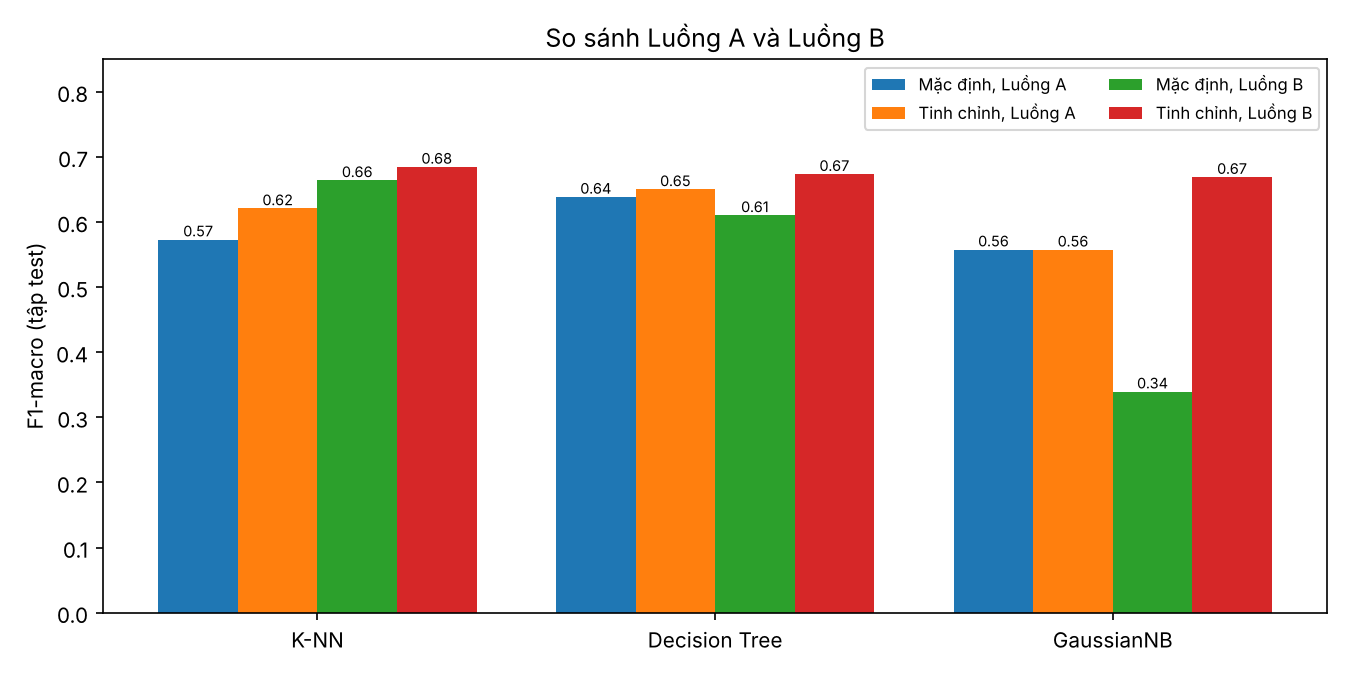
\includegraphics[width=0.8\textwidth]{res_01_compare_AB.png}
\caption{F1-macro trên tập test: mặc định và tinh chỉnh, Luồng A và Luồng B.}\label{fig:ab}\end{figure}

\subsection{Ablation: tách tác động của từng thay đổi}
\begin{table}[H]\centering\small
\begin{tabular}{@{}lcccc|cccc@{}}\toprule
 & \multicolumn{4}{c|}{CV F1-macro (tinh chỉnh)} & \multicolumn{4}{c}{F1-macro test (tinh chỉnh)}\\
Thuật toán & A & B1 & B2 & B & A & B1 & B2 & B\\\midrule
@@TABLE_ABL@@
\bottomrule
\end{tabular}\caption{Ablation: A = cơ bản; B1 = + đặc trưng mới; B2 = + One-Hot; B = cả hai.}\label{tab:abl}\end{table}
\begin{figure}[H]\centering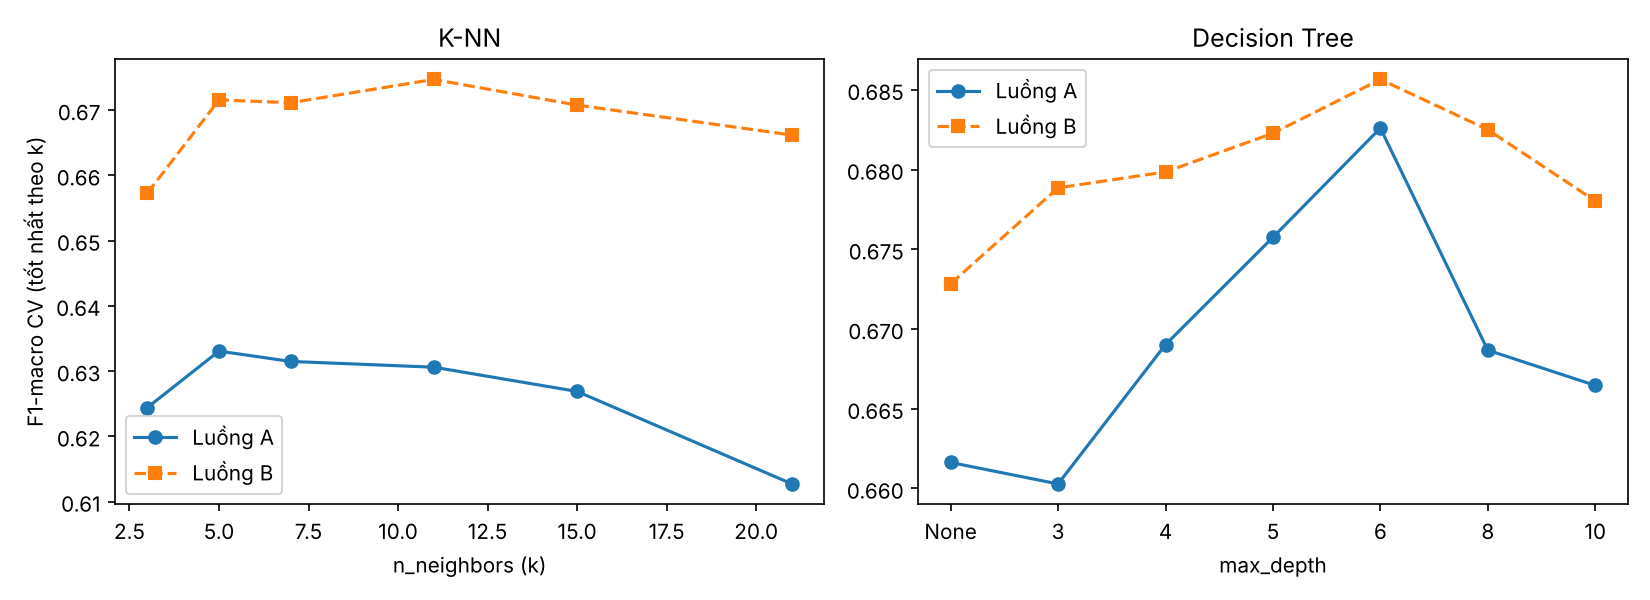
\includegraphics[width=0.95\textwidth]{res_03_sensitivity.png}
\caption{Độ nhạy tham số: F1-macro CV tốt nhất theo $k$ (K-NN) và theo \texttt{max\_depth} (Cây quyết định).}\label{fig:sens}\end{figure}

\subsection{Mô hình tốt nhất và confusion matrix}
Chọn theo F1-macro của CV (không dựa trên tập test), mô hình tốt nhất là \textbf{@@BEST_MODEL@@, Luồng @@BEST_FLOW@@}
(@@BEST_PARAMS@@): CV F1-macro @@BEST_CV@@, trên tập test Accuracy @@BEST_ACC@@ và F1-macro @@BEST_T@@. Precision/Recall theo lớp:
Dropout @@BP_Dropout@@/@@BR_Dropout@@, Enrolled @@BP_Enrolled@@/@@BR_Enrolled@@, Graduate @@BP_Graduate@@/@@BR_Graduate@@.
\begin{figure}[H]\centering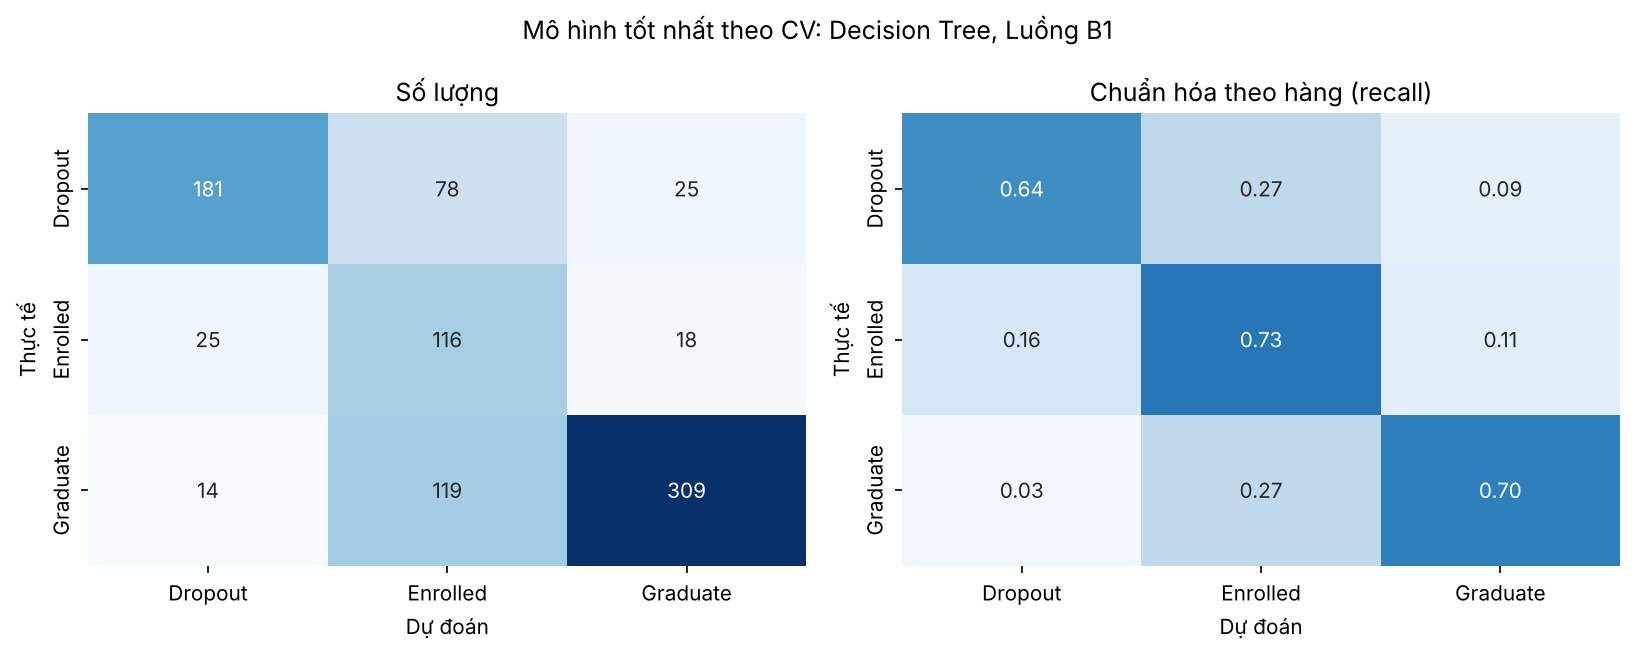
\includegraphics[width=0.95\textwidth]{res_04_confusion_best.png}
\caption{Confusion matrix của mô hình tốt nhất (số lượng và chuẩn hóa theo hàng).}\label{fig:cmbest}\end{figure}
\begin{figure}[H]\centering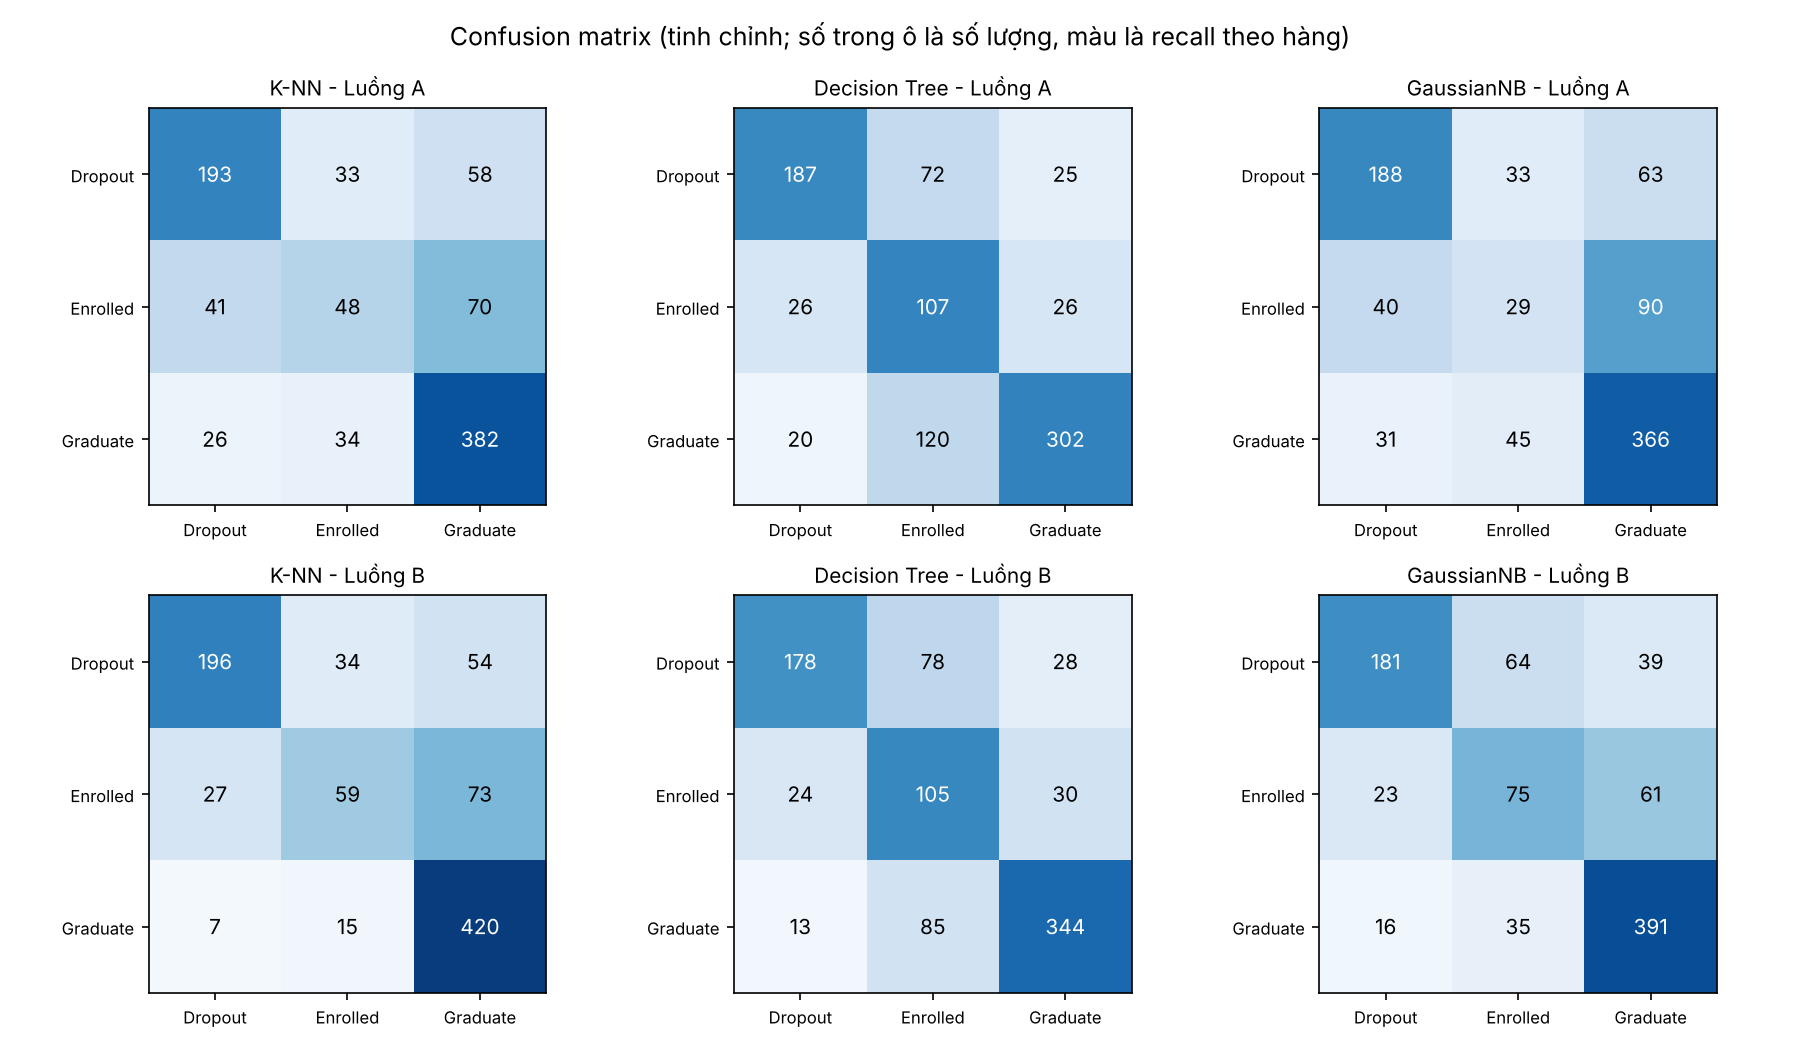
\includegraphics[width=0.95\textwidth]{res_05_confusion_grid.png}
\caption{Confusion matrix của ba thuật toán trên Luồng A và Luồng B.}\label{fig:cmgrid}\end{figure}

% =====================================================================
\section{Thảo luận và so sánh}
\subsection{So sánh Luồng A và Luồng B}
\textbf{K-NN.} F1-macro CV tăng từ @@CV_KNN_A@@ (Luồng A) lên @@CV_KNN_B@@ (Luồng B), tức @@GAIN_KNN_B@@, lớn hơn độ lệch chuẩn giữa các
fold (@@CVS_KNN_B@@); trên tập test F1-macro tăng từ @@T_KNN_A@@ lên @@T_KNN_B@@. K-NN dùng khoảng cách nên rất nhạy với cách biểu diễn:
ở Luồng A, các mã định danh (ngành, hình thức xét tuyển, nghề nghiệp) bị coi như số thực và các đặc trưng học tập chỉ ở dạng số tuyệt đối.\\
\textbf{Naive Bayes.} Tăng mạnh nhất, từ @@CV_NB_A@@ lên @@CV_NB_B@@ (CV).\\
\textbf{Cây quyết định.} CV chỉ đổi từ @@CV_DT_A@@ lên @@CV_DT_B@@ (chênh @@GAIN_DT_B@@), nhỏ hơn độ lệch chuẩn (@@CVS_DT_A@@),
nên \emph{không có bằng chứng} cho thấy Luồng B tốt hơn với thuật toán này. Điều này hợp lý vì cây quyết định tự chọn ngưỡng trên từng
cột, không phụ thuộc thang đo, và có thể tự xấp xỉ tỷ lệ bằng nhiều lần chia. Chênh lệch trên tập test (@@T_DT_A@@ so với @@T_DT_B@@) cũng
cần thận trọng: sai số chuẩn ước lượng của một tỷ lệ đo trên @@NTE@@ mẫu vào cỡ @@TEST_SE@@ trong trường hợp xấu nhất.

\textbf{Ablation (Bảng~\ref{tab:abl}).} Phần lớn mức tăng của K-NN và Naive Bayes đến từ \emph{đặc trưng tỷ lệ mới} (B1): với K-NN, B1 đạt
CV @@CV_KNN_B1@@ so với @@CV_KNN_A@@ ở A và @@CV_KNN_B@@ ở B, còn One-Hot riêng lẻ (B2: @@CV_KNN_B2@@) gần như không cải thiện. Như vậy
giả thuyết ``One-Hot giúp K-NN'' của nhóm không được ủng hộ mạnh; giả thuyết ``tỷ lệ phản ánh mức độ hoàn thành tốt hơn số tuyệt đối'' được
ủng hộ.

\subsection{Vì sao GaussianNB mặc định ``sụp đổ'' ở Luồng B?}
Với cấu hình mặc định, GaussianNB ở Luồng B chỉ đạt Accuracy @@NB_B_DEF_ACC@@ và F1-macro @@NB_B_DEF_F1@@ vì dự đoán gần như mọi mẫu là Enrolled
(Recall Enrolled @@NB_B_DEF_RENR@@). Nhóm giải thích: One-Hot tạo nhiều cột nhị phân rất thưa; với \texttt{var\_smoothing=$10^{-9}$}, phương sai của các
cột này gần bằng 0 nên một giá trị hiếm cũng tạo log-likelihood cực lớn và lấn át các cột có ích. Khi tăng \texttt{var\_smoothing} lên @@NB_B_PAR@@,
hiệu năng được khôi phục (F1-macro test @@T_NB_B@@; thử nghiệm trong notebook 03). Bài học: một cách mã hóa tốt cho thuật toán này có thể làm hỏng thuật
toán khác, nên tham số phải được tinh chỉnh theo từng luồng.

\subsection{So sánh thuật toán}
Sau tinh chỉnh, Cây quyết định có CV cao nhất ở cả hai luồng (@@CV_DT_A@@ và @@CV_DT_B@@) và ổn định (độ lệch chuẩn nhỏ), K-NN ở Luồng B có
Accuracy cao nhất (@@ACC_KNN_B@@) nhưng Recall của Enrolled thấp hơn; Naive Bayes thua ở Luồng A nhưng cạnh tranh được ở Luồng B. Các chênh lệch giữa ba mô hình
tốt nhất là nhỏ so với độ lệch chuẩn giữa các fold (từ @@CVS_DT_B@@ đến @@CVS_KNN_B@@), nên không nên khẳng định mô hình nào vượt trội tuyệt đối. Khi tinh chỉnh,
\texttt{class\_weight=balanced} làm Cây quyết định đánh đổi Accuracy lấy Recall của Enrolled (xem Bảng~\ref{tab:main}).

\subsection{Phân tích lỗi}
Với mô hình tốt nhất, @@ERR_TOTAL@@/@@NTE@@ mẫu bị dự đoán sai (Bảng~\ref{tab:conf}).
\begin{table}[H]\centering\small
\begin{tabular}{@{}lccc@{}}\toprule
Thực tế $\backslash$ Dự đoán & Dropout & Enrolled & Graduate\\\midrule
@@TABLE_CONF@@
\bottomrule\end{tabular}\caption{Confusion matrix của mô hình tốt nhất trên tập test.}\label{tab:conf}\end{table}
Lớp Enrolled có Precision thấp (@@BP_Enrolled@@) vì mô hình ``kéo'' nhiều mẫu vào lớp này: @@GRAD_TO_ENR@@ sinh viên Graduate và @@DROP_TO_ENR@@ sinh viên Dropout
bị đoán là Enrolled. Bảng~\ref{tab:err} so sánh hồ sơ trung bình của các nhóm đoán đúng và đoán sai.
\begin{table}[H]\centering\small
\begin{tabular}{@{}lrccccc@{}}\toprule
Thực tế $\to$ Dự đoán & $n$ & Môn đạt HK2 & Tỷ lệ đạt HK2 & Đóng học phí & Học bổng & Tuổi\\\midrule
@@TABLE_ERR@@
\bottomrule\end{tabular}\caption{Giá trị trung bình theo nhóm (đúng/sai) của mô hình tốt nhất.}\label{tab:err}\end{table}
\textbf{Dropout bị đoán là Enrolled} ($n=@@DE_N@@$): trung bình đạt @@DE_A2@@ môn ở học kỳ 2 (tỷ lệ đạt @@DE_RATE@@) và @@DE_FEE@@ đóng học phí đúng hạn,
trong khi nhóm Dropout được đoán đúng chỉ đạt @@DD_A2@@ môn (tỷ lệ đạt @@DD_RATE@@). Nghĩa là họ có hồ sơ học tập và tài chính giống sinh viên đang học bình thường;
các nguyên nhân thực sự (hoàn cảnh cá nhân, chuyển trường) không có trong dữ liệu, nên đây là giới hạn của dữ liệu hơn là của thuật toán.\\
\textbf{Graduate bị đoán là Enrolled} ($n=@@GE_N@@$): tỷ lệ đạt học kỳ 2 trung bình @@GE_RATE@@, thấp hơn nhóm Graduate đoán đúng (@@GG_RATE@@), và tỷ lệ có học bổng
@@GE_SCH@@ so với @@GG_SCH@@. Đây là những sinh viên tốt nghiệp nhưng có học kỳ chưa trọn vẹn, nằm sát ranh giới của Enrolled;
\texttt{class\_weight=balanced} làm ranh giới này dịch về phía Enrolled.

\subsection{Đặc trưng quan trọng}
Cây quyết định nông (Hình~\ref{fig:tree}) chia chủ yếu theo số môn đạt học kỳ 2, rồi đến tình trạng học phí. Với Cây quyết định tinh chỉnh ở Luồng B,
đặc trưng quan trọng nhất là \texttt{@@IMP1@@} (@@IMP1V@@), tiếp theo là \texttt{@@IMP2@@} (@@IMP2V@@); các đặc trưng tỷ lệ mới chiếm hạng 1 và hạng 3
(Bảng~\ref{tab:imp}), phù hợp với kết quả ablation.
\begin{figure}[H]\centering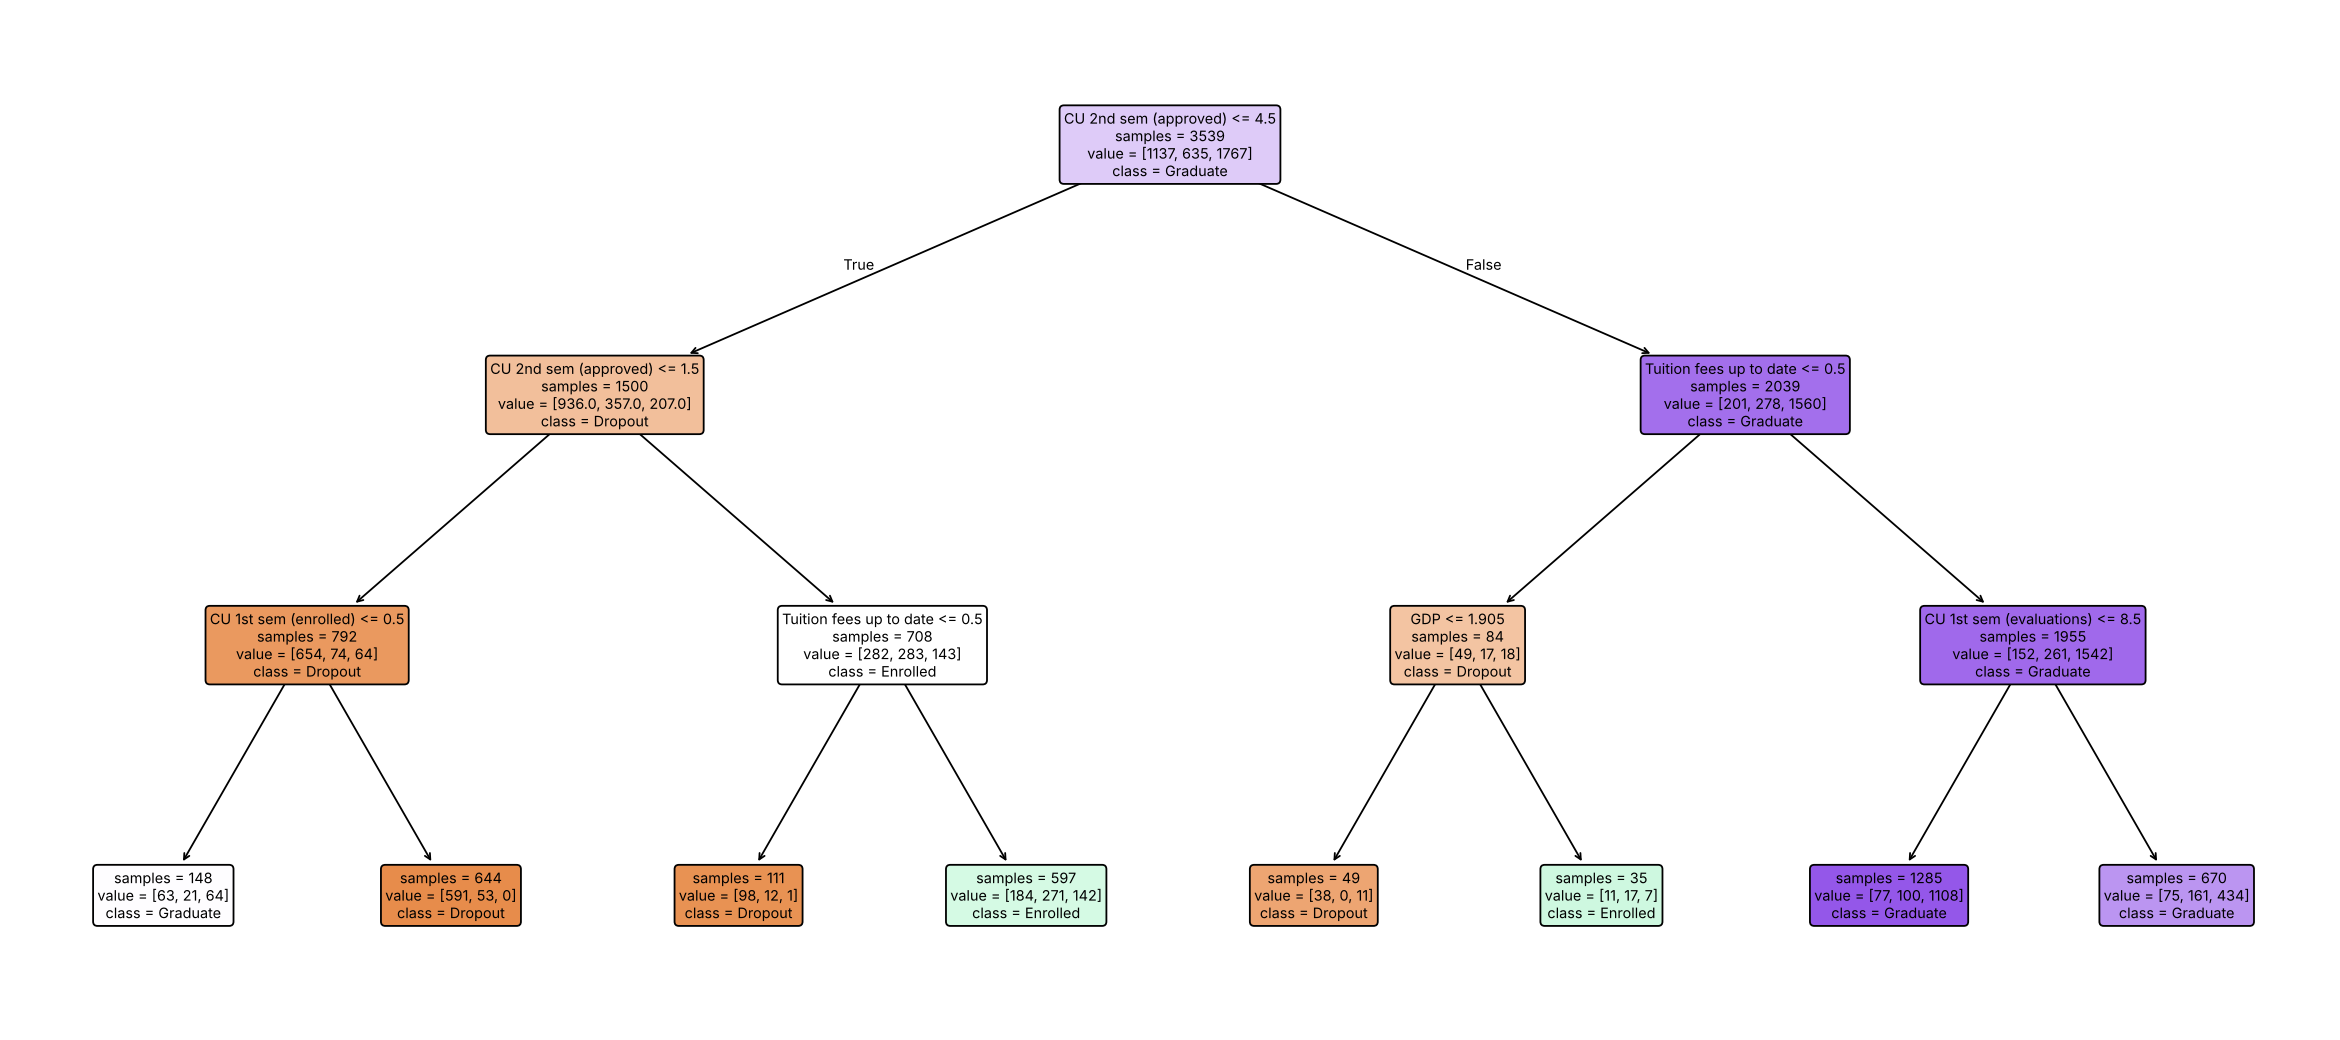
\includegraphics[width=\textwidth]{res_06_tree_depth3.png}\caption{Cây quyết định độ sâu 3 trên các cột gốc.}\label{fig:tree}\end{figure}
\begin{table}[H]\centering\small
\begin{tabular}{@{}lc@{}}\toprule Đặc trưng & Độ quan trọng\\\midrule
@@TABLE_IMP@@
\bottomrule\end{tabular}\caption{Tám đặc trưng quan trọng nhất của Cây quyết định tinh chỉnh, Luồng B.}\label{tab:imp}\end{table}

\subsection{Cấu hình cảnh báo sớm}
Đặc trưng học kỳ 2 chỉ có sau khi học kỳ 2 kết thúc, nên mô hình dùng chúng là dự đoán muộn. Nhóm chạy thêm cấu hình chỉ dùng dữ liệu nhân khẩu,
tuyển sinh, tài chính và học kỳ 1 (bỏ mọi cột \texttt{2nd sem}), cũng với GridSearchCV.
\begin{table}[H]\centering\small
\begin{tabular}{@{}llcccccc@{}}\toprule
Thuật toán & Luồng & CV F1 & Acc & F1 test (sớm) & F1 test (đầy đủ) & Giảm & Recall Dropout\\\midrule
@@TABLE_EW@@
\bottomrule\end{tabular}\caption{Cảnh báo sớm so với mô hình đầy đủ (F1 là F1-macro; Giảm = F1 đầy đủ trừ F1 sớm).}\label{tab:ew}\end{table}
F1-macro giảm khoảng @@EW_MIN@@ đến @@EW_MAX@@ so với mô hình đầy đủ; mô hình sớm tốt nhất ở Luồng B là @@EW_BEST@@.
Mức giảm vừa phải cho thấy có thể cảnh báo sớm từ cuối học kỳ 1 với độ chính xác chấp nhận được.

\subsection{Hạn chế}
(i) Dữ liệu từ một trường đại học, khó khái quát sang bối cảnh khác. (ii) Thiếu các yếu tố có thể gây bỏ học thật sự (hoàn cảnh gia đình, sức khỏe,
động lực). (iii) Kết quả báo cáo trên một lần chia train/test; độ lệch chuẩn giữa các fold (khoảng 0,01--0,02) cho thấy các chênh lệch nhỏ hơn mức này không đáng tin.
(iv) Lớp Enrolled có nhãn không phải ``kết cục cuối cùng'' nên về bản chất khó tách khỏi hai lớp còn lại. (v) Dùng giới tính, quốc tịch làm đầu vào có nguy cơ
gây thiên lệch; mô hình chỉ nên hỗ trợ tư vấn, không dùng để loại bỏ hay phân biệt đối xử với sinh viên. (vi) Xác suất của cây quyết định chưa được hiệu chỉnh.

% =====================================================================
\section{Tổng kết và hướng phát triển}
Nhóm đã xây dựng quy trình đầy đủ từ EDA đến phân tích lỗi cho bài toán dự đoán sinh viên bỏ học. Kết quả chính: (1) Cây quyết định tinh chỉnh ở
Luồng @@BEST_FLOW@@ là mô hình tốt nhất theo CV (F1-macro CV @@BEST_CV@@, test @@BEST_T@@); (2) đặc trưng tỷ lệ mới giúp rõ rệt K-NN và Naive Bayes nhưng không giúp
Cây quyết định; (3) cách mã hóa phải đi cùng tham số phù hợp (GaussianNB sụp đổ với tham số mặc định); (4) lớp Enrolled và các sinh viên Dropout ``giống sinh viên bình thường'' là
nguồn lỗi chính; (5) cảnh báo sớm chỉ dùng dữ liệu học kỳ 1 vẫn dùng được với mức giảm F1-macro khoảng @@EW_MIN@@ đến @@EW_MAX@@.

Hướng phát triển: dùng CV lặp hoặc nhiều lần chia để đánh giá chắc chắn hơn; hiệu chỉnh xác suất; thử các đặc trưng theo thời gian (xu hướng điểm) khi có dữ liệu theo tuần;
xét công bằng giữa các nhóm giới tính; thử ensemble hoặc mô hình pre-trained như phần mở rộng; và triển khai GUI trong quy trình tư vấn của nhà trường.

\begin{thebibliography}{9}
\bibitem{realinho2022} V. Realinho, J. Machado, L. Baptista, M. V. Martins, ``Predicting Student Dropout and Academic Success'', \textit{Data}, 7(11), 146, 2022.
\bibitem{sklearn} F. Pedregosa et al., ``Scikit-learn: Machine Learning in Python'', \textit{Journal of Machine Learning Research}, 12, 2825--2830, 2011.
\end{thebibliography}

\appendix
\section{Khai báo sử dụng công cụ AI}
Nhóm sử dụng Claude (Anthropic) để hỗ trợ lập kế hoạch, viết và rà soát mã nguồn (\texttt{src/}, notebook 02--04, GUI) và soạn nháp báo cáo. Các số liệu trong báo cáo được
sinh trực tiếp từ \texttt{results/} bởi \texttt{src/make\_report.py}. Nhóm chịu trách nhiệm về tính đúng đắn của nội dung và giải thích được mã nguồn, kết quả khi bảo vệ.
Nhật ký chi tiết nằm trong tệp \texttt{AI\_USAGE.md} của repository. [Nhóm bổ sung phần sử dụng AI khác nếu có.]

\section{Phân công công việc}
[Nhóm điền: thành viên nào phụ trách phần nào, theo lịch sử commit của repository.]

\end{document}
